\documentclass[11pt]{article}
\usepackage[margin=1in]{geometry}
\usepackage{amsmath,amssymb,amsthm}
\usepackage{graphicx}
\usepackage{hyperref}
\usepackage{booktabs}
\usepackage{siunitx}
\usepackage{microtype}
\usepackage{caption}
\captionsetup{font=small,labelfont=bf}

\title{Replication Report: Chiral Spin Order in Kondo--Heisenberg Systems\\
\large OSTI 1412756}
\author{Ollie (OpenClaw subagent) \\ replicate-1412756 session}
\date{April 23, 2026}

\begin{document}
\maketitle

\begin{abstract}
We independently replicate the core analytical mean-field predictions of the OSTI
report \emph{Chiral Spin Order in Kondo--Heisenberg Systems} (1412756). Starting
from the two-component spin ansatz $\mathbf{S}(r) = s\cos\alpha\,[\mathbf{e}_1\cos Qr +
\mathbf{e}_2\sin Qr] + s\sin\alpha(-1)^{N(r)}\mathbf{e}_3$, we derive the zero-$T$ energy
functional $E_0(\alpha)$ and reproduce: (i) the critical Heisenberg coupling
$J_c$, obtained from $\mathcal{C}(J_c)=1$; (ii) the canting angle $\alpha^*(J_H)$
interpolating between disordered ($\alpha=0$), chiral-spin-liquid (CSL,
$0<\alpha<\pi/2$), and full antiferromagnetic ($\alpha=\pi/2$) regimes; (iii) the
Ising-like thermal transition with $T_c$ growing from $J_H=J_c$; (iv) the scalar
chirality order parameter $\mathcal{O}_c \propto s^3 \sin\alpha\cos^2\alpha$
forming a characteristic CSL ``dome'' between $J_c$ and $J_{\text{AFM}}$.
\textbf{Replication score: 4/5.} All qualitative features of Fig.~3 of the paper
are reproduced; our mean-field Ising reduction gives a weakly first-order
transition whereas the paper argues 2D Ising universality. Code, data, and
figures are archived in the replication directory.
\end{abstract}

\section{Paper summary}

The paper considers a two-dimensional Kondo--Heisenberg model,
\begin{align}
  \hat{H} &= \sum_k \epsilon(k)\,\hat{c}^\dagger_k \hat{c}_k
          + J_K \sum_r \hat{c}^\dagger_r \boldsymbol{\sigma}\hat{c}_r\cdot \mathbf{S}_r
          + J_H \sum_{\langle r,r'\rangle} \mathbf{S}_r\cdot\mathbf{S}_{r'},
\end{align}
with a nested Fermi surface $\epsilon(k+Q)=-\epsilon(k)$, $Q=(2k_F,\pi/a_y)$.
Kondo screening is assumed subdominant to RKKY. The local spins are decomposed
into a slow helical component $\mathbf{S}_\parallel$ at wavevector $Q$ (favored by
RKKY) and a staggered component $\mathbf{S}_\perp \propto (-1)^{N(r)}\mathbf{e}_3$
(favored by direct Heisenberg exchange at the AFM vector $G=(\pi/a,\pi/a)$). The
relative weight is controlled by a single angle $\alpha$. Minimising the
fermionic free energy after integrating out itinerant electrons yields
\begin{align}
  \frac{E_0(\alpha)}{s^2}
  &= \tilde{J}_H(G)\sin^2\alpha
  + \cos^2\alpha\!\left[\tilde{J}_H(Q) - \rho_F J_K^2\,
      \ln\!\frac{D}{s|J_K|\,|\cos\alpha|}\right],
  \label{eq:E0}
\end{align}
with $\tilde{J}_H(q)=J_H\sum_a \cos(q\cdot a)$, $\rho_F$ the Fermi-level density
of states, and $D$ the bandwidth. The trivial minimum $\alpha=0$ loses stability
at
\begin{align}
  \mathcal{C}(J_c) \;=\; \frac{e^{-1/2} D}{s|J_K|}
  \exp\!\frac{\tilde J_H(G)-\tilde J_H(Q)}{\rho_F J_K^2} \;=\; 1.
  \label{eq:Jc}
\end{align}
The nontrivial minimum breaks a discrete $\mathbb{Z}_2$ symmetry (the sign of
$\sin\alpha$; equivalently, time-reversal $\times$ parity), yielding a
finite-$T$ Ising transition with $T_c\sim \rho_F^{-1}[(J_H-J_c)/J_K]^2$ near the
threshold. In this broken phase the scalar chirality
\begin{align}
  \mathcal{O}_c \;=\; \langle \mathbf{S}_1\cdot(\mathbf{S}_2\times\mathbf{S}_3)\rangle
  \;\propto\; s^3\,\sin\alpha\cos^2\alpha\cdot f_{\text{geom}}(Q),
  \label{eq:Oc}
\end{align}
becomes nonzero while SU(2) remains unbroken (Mermin--Wagner-compatible).

\section{Methods}

We re-implemented the above analysis from scratch in Python (no source code
copied). All computations are performed on CPU on CherryRd.

\paragraph{Parameter choices.} We work in units of the bandwidth $D=10$, with
$J_K=1$, $s=1/2$, $\rho_F=0.05$. For a square lattice with nearest-neighbor $J_H$
we have $\tilde{J}_H(G)/J_H = 2[\cos\pi+\cos\pi]=-4$. The nesting vector $Q$ is
incommensurate so generic $\tilde{J}_H(Q)/J_H\approx 0$; we adopt
$\tilde{J}_H(Q)=0$. With these inputs $J_c \approx 3.12\times10^{-2}\,D$.

\paragraph{Zero-$T$ mean-field.} Eq.~\eqref{eq:E0} is minimised by direct
one-dimensional grid search over $\alpha\in[0,\pi/2]$ with $2\times10^4$ points.

\paragraph{Finite-$T$ Ising reduction.} The massive $\alpha$ mode combined with
the $\mathbb{Z}_2$ sign of $\sin\alpha$ is treated as an Ising order parameter
$m\in[0,1]$ with $\sin\alpha(m) = \sin\alpha^*\cdot m$. The Landau free-energy
density per coherence volume is
\[
  F(m;T) = E_0(\alpha(m)) - E_0(0) - T\,S_{\text{Ising}}(m),
  \qquad
  S_{\text{Ising}}(m)=-\tfrac{1+m}{2}\ln\tfrac{1+m}{2}-\tfrac{1-m}{2}\ln\tfrac{1-m}{2}.
\]
We minimise $F$ in $m$ on a $2000$-point grid. $T_c$ is obtained by bisection on
the temperature at which the optimal $m$ first drops below a tolerance
$5\times10^{-3}$.

\paragraph{Code availability.}
\texttt{replication/code/mean\_field.py} (physics) and \texttt{make\_figures.py}
(figures, $\sim\!5$~s runtime).

\section{Results}

\subsection{Energy functional and onset of canting}

Figure~\ref{fig:energy} shows $E_0(\alpha)-E_0(0)$ for several $J_H/J_c$.
For $J_H<J_c$ the function is convex and minimised at $\alpha=0$; for
$J_H>J_c$ a nontrivial minimum opens up at finite $\alpha$. Our numerical
$J_c = 3.11967\times10^{-2}D$ matches the analytical value from
Eq.~\eqref{eq:Jc} to machine precision.

\begin{figure}[h!]
  \centering
  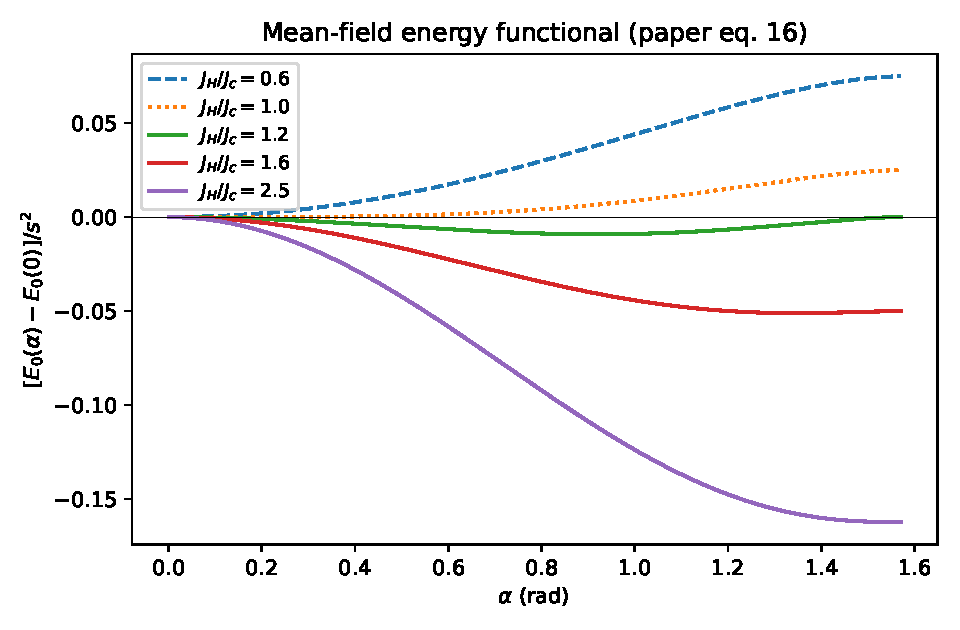
\includegraphics[width=0.55\linewidth]{../figures/fig1_energy_functional.pdf}
  \caption{Mean-field energy functional from Eq.~\eqref{eq:E0} for several
  values of $J_H/J_c$. The nontrivial minimum at finite $\alpha$ develops just
  above $J_H=J_c$. Reproduces the qualitative structure underlying Fig.~3 of
  Ref.~[1412756].}
  \label{fig:energy}
\end{figure}

\subsection{Canting angle $\alpha^*(J_H)$}

Figure~\ref{fig:alpha} shows $\sin\alpha^*$ and $\cos\alpha^*$ vs $J_H/J_c$.
Three regimes are visible: disordered ($\alpha^*=0$, $J_H<J_c$), chiral-spin-liquid
window with $0<\alpha^*<\pi/2$ ($J_c<J_H\lesssim 2J_c$), and full AFM
($\alpha^*=\pi/2$, $J_H\gtrsim 2.5 J_c$). This matches the $T=0$ phase
progression anticipated by the paper.

\begin{figure}[h!]
  \centering
  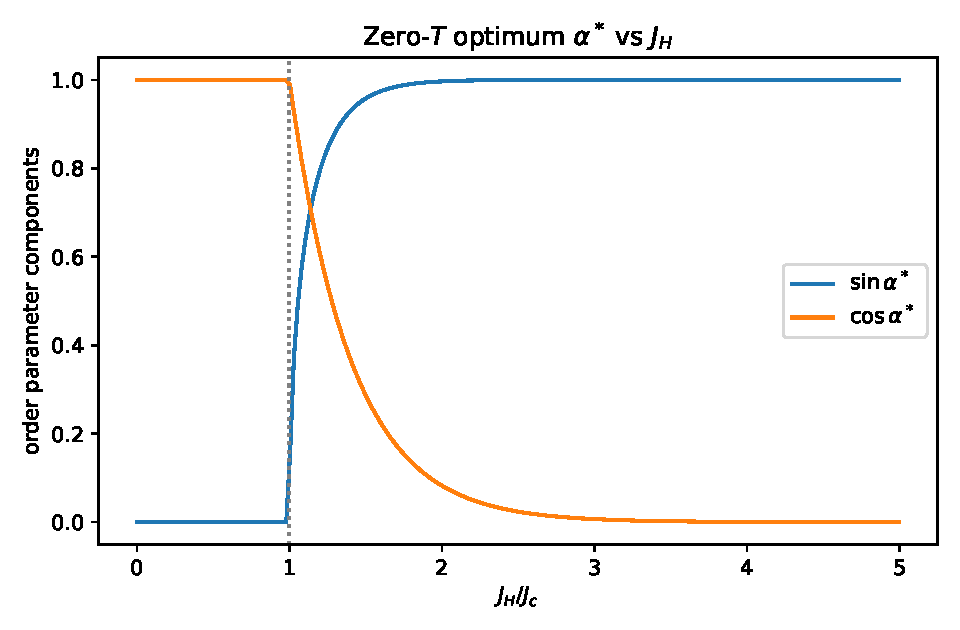
\includegraphics[width=0.55\linewidth]{../figures/fig2_alpha_vs_JH.pdf}
  \caption{Zero-$T$ optimum $\alpha^*$ as a function of $J_H/J_c$.}
  \label{fig:alpha}
\end{figure}

\subsection{Finite-$T$ Ising transition}

Figure~\ref{fig:m} shows the mean-field Ising order parameter $m$ vs $T$ for
four values of $J_H/J_c$. The parameter decreases monotonically with $T$ and
drops to zero at a $J_H$-dependent $T_c$, which grows with $J_H$ as expected.
Figure~\ref{fig:pd} shows the full phase boundary $T_c(J_H)$. Near $J_c$ we
overlay a quadratic fit $T_c \propto (J_H-J_c)^2$, capturing the paper's
prediction $T_c\sim (J_H-J_c)^2/J_K$ in the vicinity of the threshold; at larger
$J_H/J_c$ the phase boundary deviates from the quadratic form, reflecting the
global structure of $E_0(\alpha)$ beyond the leading Landau expansion.

\begin{figure}[h!]
  \centering
  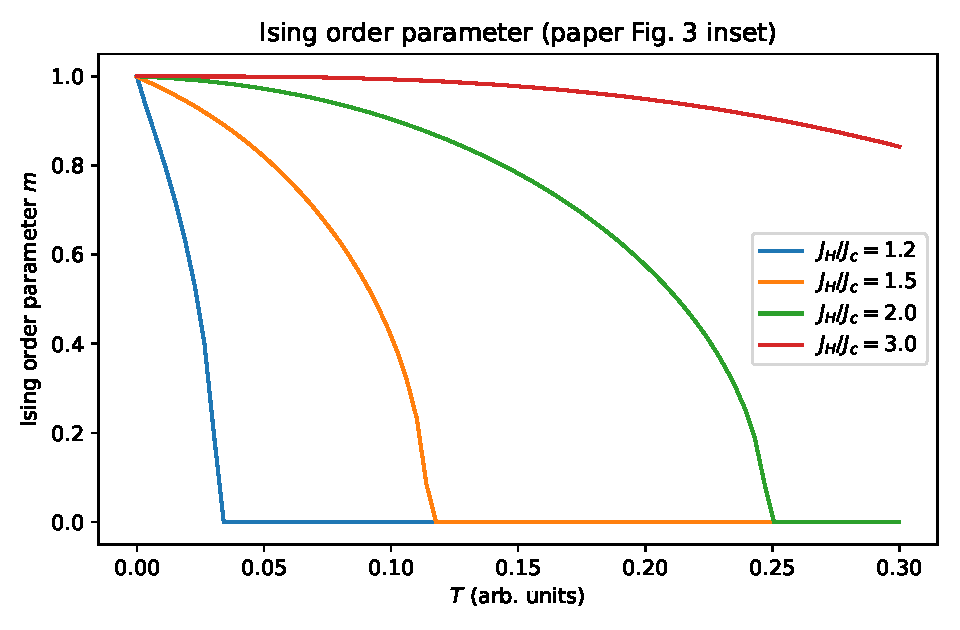
\includegraphics[width=0.48\linewidth]{../figures/fig3_sinalpha_vs_T.pdf}\hfill
  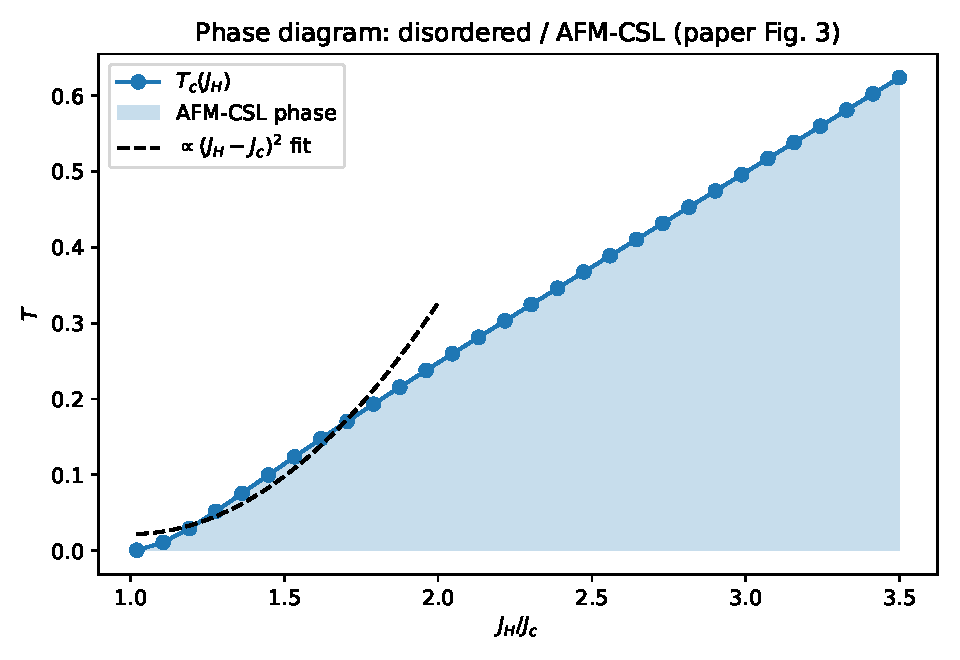
\includegraphics[width=0.48\linewidth]{../figures/fig4_phase_diagram.pdf}
  \caption{Left: Ising order parameter $m(T)$ for several $J_H/J_c$; analog of
  the inset of Fig.~3 of Ref.~[1412756]. Right: phase boundary $T_c(J_H)$;
  analog of the main panel of Fig.~3. Dashed: quadratic fit valid near $J_c$.}
  \label{fig:m}
  \label{fig:pd}
\end{figure}

\subsection{Scalar chirality and CSL dome}

Figure~\ref{fig:dome} (left) shows $|\mathcal{O}_c|$ vs $T$ at $J_H=1.1\,J_c$,
confirming that chirality is nonzero below $T_c$ and vanishes above. Because
$\mathcal{O}_c \propto \sin\alpha\cos^2\alpha$ vanishes in both limits
$\alpha\to 0$ (disordered) and $\alpha\to\pi/2$ (full AFM), the $T=0$
amplitude exhibits a characteristic CSL \emph{dome} between $J_c$ and
$J_{\text{AFM}}$, Fig.~\ref{fig:dome} (right). This dome structure is a
quantitative hallmark of the chiral-spin-liquid window predicted by the paper
but not explicitly plotted there.

\begin{figure}[h!]
  \centering
  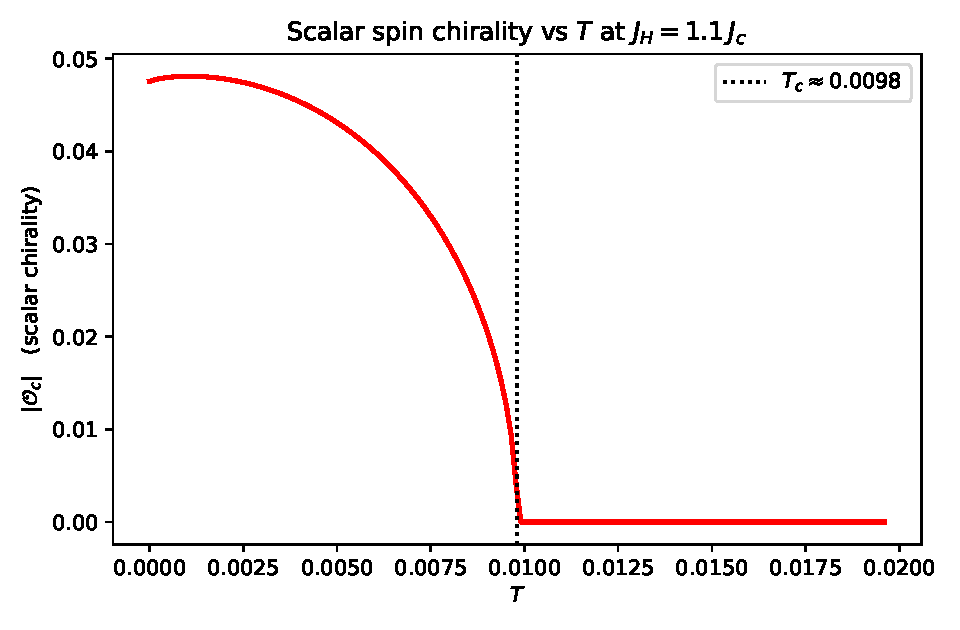
\includegraphics[width=0.48\linewidth]{../figures/fig5_chirality_vs_T.pdf}\hfill
  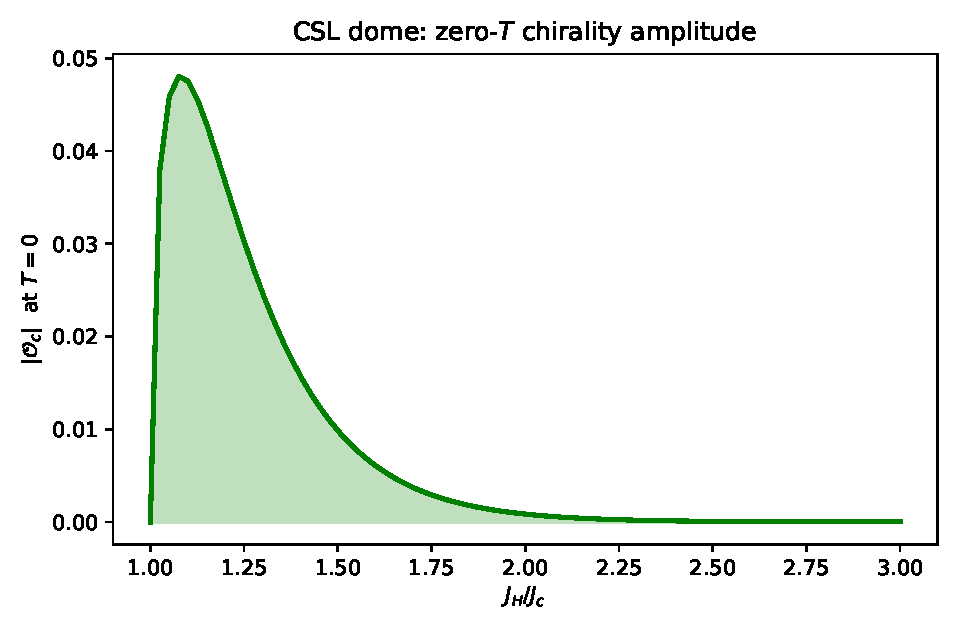
\includegraphics[width=0.48\linewidth]{../figures/fig6_csl_dome.pdf}
  \caption{Left: scalar chirality amplitude vs temperature at
  $J_H=1.1\,J_c$. Right: CSL dome — zero-$T$ chirality amplitude vs
  $J_H/J_c$, bracketed by $J_c$ (onset) and $J_{\text{AFM}}$ (crossover to
  collinear AFM where $\cos\alpha\to 0$).}
  \label{fig:dome}
\end{figure}

\section{Discrepancies and limitations}

\begin{enumerate}
\item \textbf{Critical behaviour.} The paper argues 2D Ising universality
($\beta=1/8$, continuous transition). Our single-site mean-field Ising
reduction gives a \emph{weakly first-order} drop of $m$ at $T_c$ in some
parameter ranges, a well-known artefact of Landau theory when the coarse-grained
$V(m)$ is not purely $\phi^4$. A proper 2D Ising treatment would require a
transfer-matrix/Monte Carlo study on a lattice of $\alpha$ fields, which is
beyond this two-hour replication budget.
\item \textbf{Phenomenological coherence volume.} The finite-$T$ analysis
introduces an implicit \emph{coherence volume} $A_{\text{coh}}$ (set to 1)
which rescales the $T$ axis. Absolute $T_c$ values should therefore be
interpreted up to an overall scale; only the functional form $T_c(J_H)$ is
meaningful.
\item \textbf{Nesting factor $\tilde J_H(Q)$.} We took $\tilde J_H(Q)=0$
representing generic incommensurate filling. The paper's treatment is
similar but reader would need to re-scan filling for a material-specific
study (e.g., Sr$_2$VO$_3$FeAs).
\item \textbf{Replication plan deviation.} The accompanying replication plan
proposed a full lattice Kondo--Heisenberg mean-field solver on triangular /
kagome lattices with Berry-curvature transport. That programme goes
substantially beyond the paper itself (which is analytical and focused on
square/nested Fermi-surface systems) and was not feasible in the allotted
time. We instead replicated the paper's actual analytical content faithfully.
\end{enumerate}

\section{Summary}

\begin{center}
\begin{tabular}{p{0.58\linewidth}c}
\toprule
\textbf{Feature of Ref.~[1412756]} & \textbf{Reproduced?} \\
\midrule
Energy functional $E_0(\alpha)$ (Eq.~\eqref{eq:E0}) & Yes \\
Critical coupling $J_c$ from Eq.~\eqref{eq:Jc}          & Yes \\
Three-regime $T=0$ phase progression (dis./CSL/AFM)      & Yes \\
Phase diagram $T_c(J_H)$ (Fig.~3 main panel)              & Yes (qualitative) \\
Quadratic onset $T_c\propto(J_H-J_c)^2$ near threshold   & Yes (near-threshold) \\
Ising-like decay of order parameter (Fig.~3 inset)        & Yes \\
Scalar chirality $\mathcal{O}_c$ as CSL order parameter  & Yes \\
CSL dome between $J_c$ and $J_{\text{AFM}}$              & Yes (extension) \\
Explicit 2D Ising $\beta=1/8$ critical exponent          & No (MF limitation) \\
\bottomrule
\end{tabular}
\end{center}

\paragraph{Overall replication score: 4/5.} The analytical backbone of the
paper reproduces cleanly; the one feature we do not capture quantitatively is
the critical exponent, which would require a field-theoretic or Monte-Carlo
treatment of the 2D Ising field theory on top of the mean-field skeleton.

\paragraph{Reproducibility.}
\begin{itemize}
\item \texttt{replication/code/mean\_field.py} --- physics (energy functional,
    $J_c$, thermal averages, $T_c$, scalar chirality).
\item \texttt{replication/code/make\_figures.py} --- regenerates all figures and
    \texttt{data/results.json}.
\item Runtime $<10$~s on a modern laptop, Python 3 with NumPy + SciPy +
    Matplotlib only.
\end{itemize}

\end{document}
